% -*- root: ../root.tex -*-
\section[Lecture 2]{The Uniquness  Thoerem} % (fold)
\label{sec:lecture_2}

\subsubsection*{The Uniqueness Theorem} % (fold)
\label{ssub:the_uniqueness_theorem}
The problem is that we would like to say something about then two measures on the same measurable space \(\X,\E\) on ``many'' sets (e.g. the the power set). E.i, when \(\mu(A)=\upsilon(A)\).

We cannot check all sets in \(\E\). So we would like to say something about how many sets we need to check to astablish that \(\mu(A)=\upsilon(A)\) for all \(A\in\E\)?

For some paving \(\D\) and a \(\E=\sigma(\D)\) and two measures \(\mu\) and \(\upsilon\) we want to show that if \(\mu(D)=\upsilon(D)\, \forall \, D\in \D\) then it also holds that \(\mu(A)=\upsilon(A)\, \forall \, A\in \E\) trick is to:
\begin{enumerate}
  \item Show that \(\mu(D)=\upsilon(D)\, \forall \, D\in\D\)
  \item Then construct a set \(\sH=\{A\in\E\mid \mu(A)=\upsilon(A)\}\supset\D\)
  \item Then show that \(\sH=\E\)
\end{enumerate}

The last part is however not easy unless we can show that \(\sH\) is a \(\sigal\). So instead we make a loser requirement on \(\sH\) and then try to show that \(\sH=\E\) given some stronger requirements on \(\D\) than just being a generator for the \(\sigal\).
\begin{defn}
A paving \(\sH\) os a set \(\X\) is a \important{Dynkin class} if
\begin{enumerate}
  \item \(\X\in\sH\) (the same as \(\sigma\)-algebra)
  \item \(A,B\in\sH,\, A\subset B \Rightarrow B\setminus A\in \sH\) (stronger than the \(\sigma\)-algebra but as \(\X\setminus A=A^c\) then it is also stable under complements)
  \item \(\nset{A}\in\sH,\, \nsubseti{A} \Rightarrow \bigcup_{n=1}^\infty A_n\) (looser than \(\sigma\)-algebra)
\end{enumerate}
\end{defn}
To show that a Dynkins class is af \(\sigma\)-algebra and vice-versa we need to lemmas
\begin{lem}
if \(\A\) is an algebra it holds that
\[
  A,B\in\A \Rightarrow A\setminus B\in \A
\]
\end{lem}
\begin{lem}
If \(\E\) is a \(\sigma\)-algebra it is also an algebra
\end{lem}
So the property that \(A,B\in\A \Rightarrow A\setminus B\in \A \) also holds for a \(\sigma\)-algebra.

We then introduce a new lemma that states \(\E=\sH\) and that \(\sH=\E\).
\begin{lem}
 If \(\E\) is a \(\sigma\)-algebra, then \(\E\) is also a Dynkins Class. If \(\sH\) is a Dynkins class which is stable under intersections, then \(\sH\) is a \(\sigma\)-algebra.
 \end{lem}
 \begin{proof}
 The first part follows easlialy. (1) is the same for both (2) follows from the two lemmas stating that if \( A,B\in\A \Rightarrow A\setminus B\in \A\) holds for a \(\sigma\)-algebra. (3) holds, as a \(\sigma\)-algebra is stable under all types of unions, also unions of increasing sets. To show that \(\sH\) which is \(cap\)-stabe  is a \(\sigma\)-algebra we first note that a DC which is stable under \(\cap\) is also stable  under finite \(\cup\): if \(A,B\in\sH\) then
 \[
   A\cup B=(A^c\cap B^c)^c\in\sH
 \]
 if \(\nseti{A}\in\sH\), we let
 \[
   B_n=A_1\cup\ldots\cup A_n
 \]
 As a \(\cap\)-stable DC is stable under finite unions, then \(B_n\in\sH\). And as \(\nsubseti{B}\) we have that \(\bigcup_{n=1}^\infty B_n\in\sH\). But
 \[
   \bigcup_{n=1}^\infty B_n=\bigcup_{n=1}^\infty A_n
 \]
 \end{proof}
So if a DC \(\sH\) is \(\cap\)-stable it is in fact a \(\sigma\)-algebra.
\begin{rem}
If \((\sH_i)_{i\in I}\) is a family of DC, the intersection \(\bigcap_{i\in I}\sH_i\) is also a DC
\end{rem}
\begin{rem}
A DC generated by \(\D\) is the smallest DC containg all the elements of \(\D\)
\end{rem}
\begin{lem}[\index{Dynkins lemma}Dynkins lemma]
Let \(\D\subset\sH\subset\E\) be pavings on the set \(\X\), and assume that \(\E=\sigma(\D)\). If \(\D\) is \(\cap\)-stable, and if \(\sH\) is a DC, then \(\sH=\E\).
\end{lem}
\begin{proof}
Let \(\K\) be the smallest DC containing \(\D\). Then
\[
  \D\subset\K\subset\sH\subset\E
\]
The proof is to show that \(\K\) is \(\cap\)-stabel. If this is true, then it follows from above lemma that \(\K\) is a \(\sigma\)-algebra. As \(\E\) is the smallest \(\sigma\)-algebra containing \(\D\) and \(\K\) is a \(\sigma\)-algebra contaning \(\D\) than it must be true that \(\K=\E\). As \(\sH\) is squezzed between \(\K\) and \(\E\) then \(\sH=\E\). E.i. \(\sH\) is a \(\sigma\)-algebra.

The proof follows as
\begin{enumerate}
  \item Show that \(\K\) is \(\cap\)-stabel

for each \(A\in\K\), introduce a new paving
\[
  \K_A=\left\{ B\in\K\mid A\cap B\in \K\right\}
\]
\(\K_A\) is a DC as
\begin{enumerate}[label=(\alph*)]
  \item \(\X\in\K_A\) as \(A\cap\X \Rightarrow A\subset\D\subset\K\). As \(\K_A\) is the intersection of all elements of \(\K\) and \(\X\) is a element of \(\K\)
  \item \(\tilde{A},B,\tilde{A}\subset B \Rightarrow B\setminus\tilde{A}\in\K_A\). Then \(\tilde{A}\cap A, B\cap A\in \K\) with \(\tilde{A}\cap A\subset B\cap A \). So
  \[
    (B\setminus\tilde{A})\cap A=\underbrace{(B\cap A)}_{\in\K}\setminus \underbrace{(\tilde{A}\cap A)}_{\in\K}
  \]
So \(B\setminus\tilde{A}\in\K\)
\item \(\nseti{B}\in\K_A,\, \nsubseti{B} \Rightarrow \bigcup_{n=1}^\infty B_n \in\K_A\)
\[
  A\cap \bigcup_{n=1}^\infty B_n=\bigcup_{n=1}^\infty\underbrace{(A\cap B_n)}_{\in\K}
\]
as \(\K\) is a DC. Further \(\nsubseti{A\cap B}\), so \(\bigcup_{n=1}^\infty A\cap B_n\in\K_A\)
\end{enumerate}
\end{enumerate}
\begin{enumerate}[resume]
  \item Note that \(\D\subset\K_A\subset\K\) and for \(A,B\in\D\), then \(A\cap B\in\D\subset \K\) which can given the definition of \(\K_A\) this can be reformulated as: if \(A\in\D\), then \(\D\subset\K_A\) we must have that \(\K_A=\K\). \(\K\) is the smallest DC that contains \(\D\) and \(\D\subset\K_A\), then \(\K_A=\K\). And a \(\K_A\) is defined by the intersections of \(\K\) then \(\K\) is \(\cap\)-stabel.
\end{enumerate}
\begin{figure}[htbp]
  \centering
  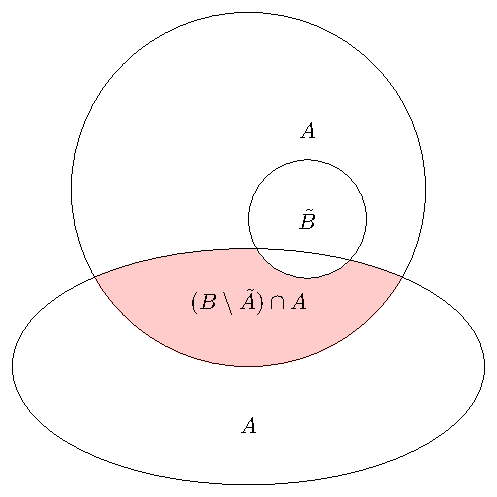
\includegraphics[width=0.5\textwidth]{fig/intersec.pdf}
  \caption{The \((B\setminus\tilde{A})\cap A\) }
  \label{fig:label}
\end{figure}
\end{proof}
Using the above we can then prove the \important{uniqueness theorem for!probability measures}. The steps are as follows
\begin{enumerate}
  \item Let \(\upsilon,\mu\) be two measures of probability on a measurable space, and assume that \(\E=\sigma(\D)\) and that
  \[
    \mu(D)=\upsilon(D)
  \]
if \(\D\) is \(\cap\)-stabel, then \(\mu=\upsilon\).
  \item contruct a paving where the two measures are equal
  \[
    \sH=\{F\in\E\mid \mu(F)=\upsilon(F)\}
  \]
  and show that \(\sH\) is a DC. This can be done with Dynkins lemma, which requires that
  \begin{enumerate}
    \item That \(\D\) is \(\cap\)-stabel follows by the theorem
    \item establish that \(\D\subset\sH\subset\E\). But this clearly follows from the contruction of \(\sH\)
    \item Then all we need to show is that \(\sH\) is a DC
  \end{enumerate}
  To show that \(\sH\) is a DC we note that
  \begin{itemize}
    \item As \(\mu,\upsilon\) are probability measures, then clearly \(\X\in\sH\).
    \item If \(A\subset B\) are two \(\sH\) sets, then
    \[
      \mu(B\setminus A)=\mu(B)-\mu(A)=\upsilon(B-\upsilon(A))=\upsilon(B\setminus A)
    \],
    so \(B\setminus A\in\sH\)
    \item If \(\nsubseti{F}\in\sH\), then
    \[
      \mu\left(\bigcup_{n=1}^\infty F_n\right)=\lim_{n \rightarrow\infty} \mu(F_n)=\lim_{n \rightarrow\infty}\upsilon(F_n)=\upsilon\left(\bigcup_{n=1}^\infty F_n\right)
    \],
    then \(\bigcup_{n=1}^\infty F_n\in\sH\)


  \end{itemize}

\end{enumerate}
\subsection{Product Algebra} % (fold)
\label{ssub:product_algebra}
Looks a \(\sigma\)-algebra generated by several maps. That is, if you have many measurable maps and you take the cartisan product, will the product then still be measurable.
% subsubsection product_algebra (end)
\subsection{Measurability of intergrals} % (fold)
\label{sub:measurability_of_intergrals}
Examine under what conditions a integral is measurable
% subsection measurability_of_intergrals (end)
\subsection{Measurable maps} % (fold)
\label{sub:measurable_maps}
\begin{defn}\label{measurable_map}
Lad \(\X,\E\) and \(\Y,\K\) be two measurable spaces, and let \(f:\X \rightarrow \Y\) be a map. We say that \(f\) is \important{measurable} if
\[
  f^{-1}(B)\in\E \text{ for all } B\in\K
\]
\end{defn}
\begin{rem}
We say that a \(f\) is \(\E-\K\) measurable if it satifies above
\end{rem}
\begin{rem}
If there is no confusion about which algebra to use, we say that either \(f\) is \(\E\)-measurable if the \(\sigma\)-algebra \(\Y\) is fixed and the only choice of confusion is the \(\sigma\)-algebra on \(\X\). Similary we may say that that \(f\) is \(\K\) measurable if \(\X\) is fixed, and the only possible confusion is the choice of \(\sigma\)-algebra on \(\Y\)
\end{rem}
Often we cannot check all the sets in the \(\sigma\)-algebra as many of them are not acceseable for direct description. Luckly we only have to check the condition given in \cref{measurable_map} on the generator for for the \(\sigma\)-algebra.

\begin{lem}
Let \((\X,\E)\) and \(\Y,\K\) be two measurable spaces, and let \(f:\X \rightarrow \Y\) be a map. Let \(\D\) be a paving on \(\Y\) and assume that \(\K=\sigma(\D)\) . If
\[
  f^{-1}(D)\in\E\, \forall\, D\in\D,
\]
then \(f\) is \(\E-\K\)-measurable
\end{lem}
% subsection measurable_maps (end)
\subsection{Product measures} % (fold)
\label{ssub:product_measures}
Thw product of two finite measures \(\mu\otimes\upsilon\) is agian a measure. Especially: the product of two probability measures is agian a probability measure.

\begin{them}
Let \((\X,\E, \mu)\) and \(\Y,\K, \upsilon\) be \(\sigma\)-finite spaces. Then there is a unique measure \(\mu\otimes\upsilon\) on the product space \(\X\times\Y, \E\otimes\K\) satesfying that
\[
  \mu\otimes\upsilon(A\times B)=\mu(A)\upsilon(B)\quad A\in\E,B\in\K
\]

\end{them}